% Chapter Template

\chapter{Results and Conclusion}\doublespacing % Main chapter title

\label{Chapter7} % Change X to a consecutive number; for referencing this chapter elsewhere, use \ref{ChapterX}

\lhead{Chapter vii. \emph{Results}} % Change X to a consecutive number; this is for the header on each page - perhaps a shortened title


% --------------------------------
% Study Summary
% --------------------------------

\section{Results}

\begin{figure}[htbp]
  \centering
  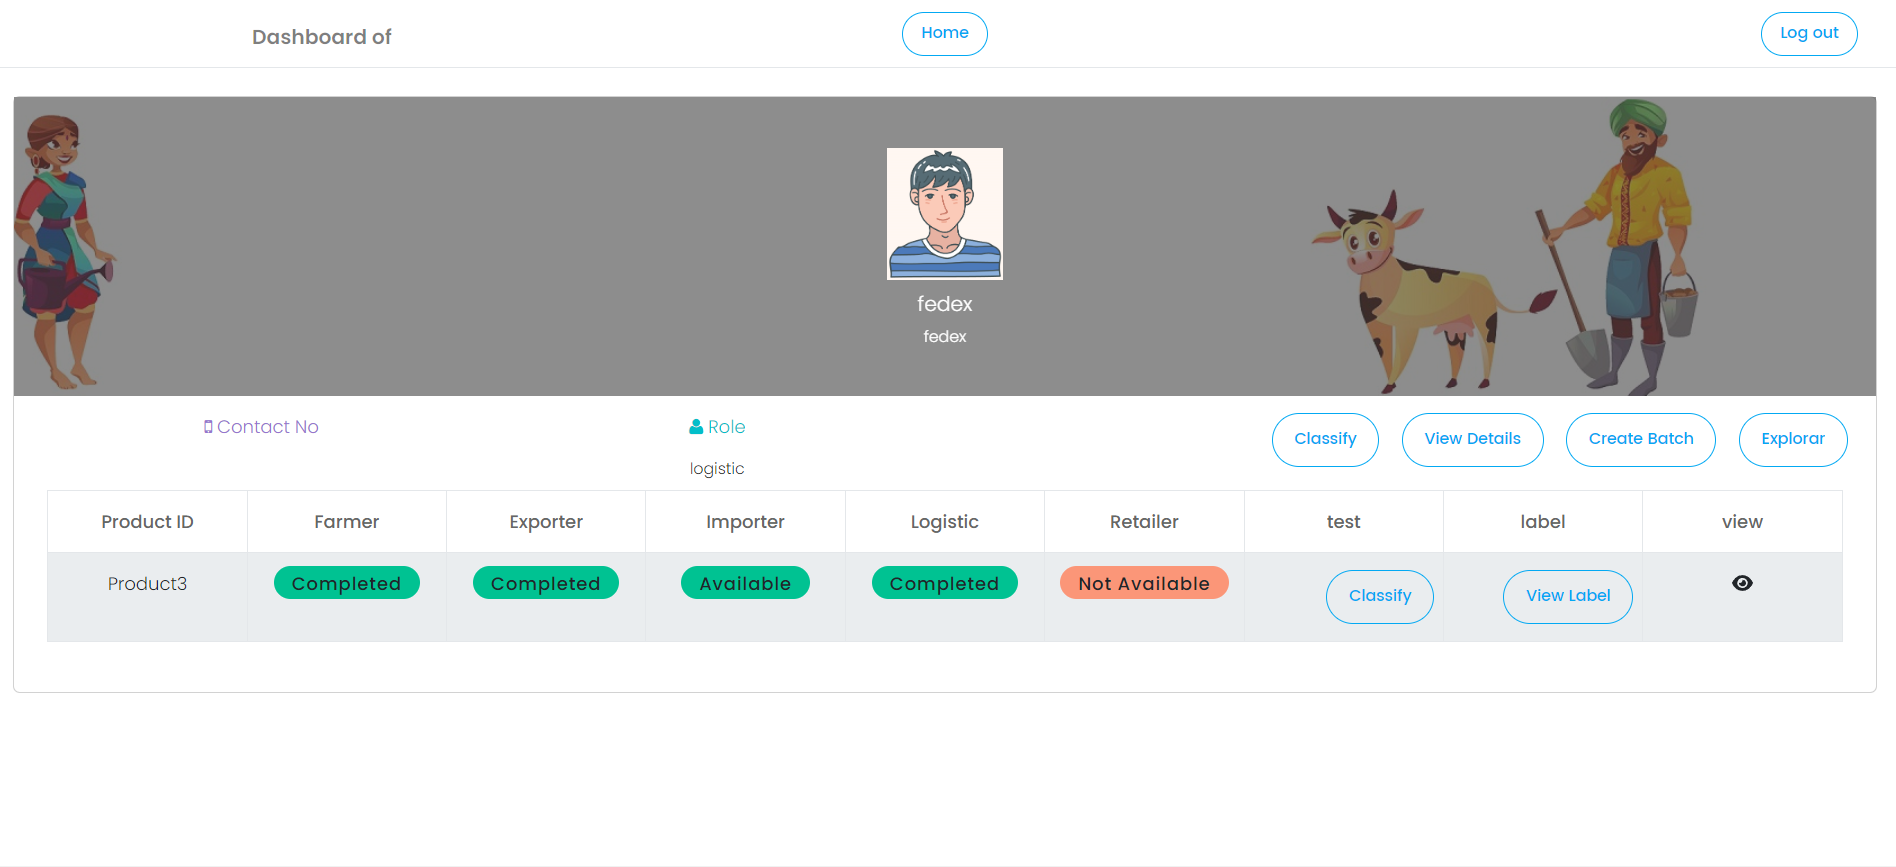
\includegraphics[width=0.9\textwidth]{Chapters/Chapter_7/images/User_interface.png}
  \caption{User Interface }
  \label{fig:figure7_1}
  \end{figure}
\noindent {The Results obtained from  our project is shown with different diagrams provided below\par}
\noindent{The provided user dashboard interface shown in Figure \ref{fig:figure7_1} offers a visually appealing and user-friendly layout for managing products within a supply chain system. Here's a description of the various sections and functionalities:
\begin{itemize}
   \item User Information Section:
   \begin{itemize}
      \item At the top of the dashboard, there is a background image with an overlay.
      \item Within the overlay, the user's profile picture, name, and address are displayed.
      \item If the user has uploaded a profile picture, it is shown; otherwise, a default image is used.
   \end{itemize}
   \item User Details Section:
   \begin{itemize}
      \item Below the user information, there are sections displaying the user's contact number and role within the system.
      \item These details provide quick access to essential user information.
   \end{itemize}
   
   \item Action Buttons:
   \begin{itemize}
      \item The dashboard includes three action buttons: "Explore," "Create Batch," and "View Details."
      \item Clicking the "Explore" button takes the user to a page for exploring products.
      \item The "Create Batch" button opens a dialog or form for creating a new batch of products.
      \item The "View Details" button allows users to access more detailed information about the system.
   \end{itemize}
   \item Product Classification Component:
   \begin{itemize}
      
      \item A component related to product classification is present on the dashboard.
      \item This component likely provides options or tools for classifying products based on specific criteria.
   \end{itemize}
   \item Product Overview Table:
   \begin{itemize}
      
      \item The main section of the dashboard features a table presenting an overview of the products.
      \item Each row in the table represents a specific product and contains several columns.
      \item The columns include the product ID and the parties involved in the supply chain, such as farmers, exporters, importers, logistic providers, and retailers.
      \item There are also columns labeled "test," "label," and "view."
   \end{itemize}
   \item Dynamic Content and Interactions:
   \begin{itemize}

\item The content in the columns of the table dynamically changes based on the product's status and role within the supply chain.
\item Different labels or status indicators, such as "Completed," "Processing," or "Not Available," are displayed to represent the current stage or availability of the product at each role.
\item Users can interact with the table by clicking on specific elements.
\item For example, clicking on the "View" column triggers an action to view more detailed information about the selected product.
\end{itemize}
\end{itemize}
In summary, this user dashboard provides an intuitive interface for managing products within a supply chain system. It offers easy access to user information, various functionalities for product management, and a comprehensive overview of products and their statuses.\par }
\begin{figure}[ht]
  \centering
  \begin{minipage}[b]{0.6\linewidth}
    \centering
    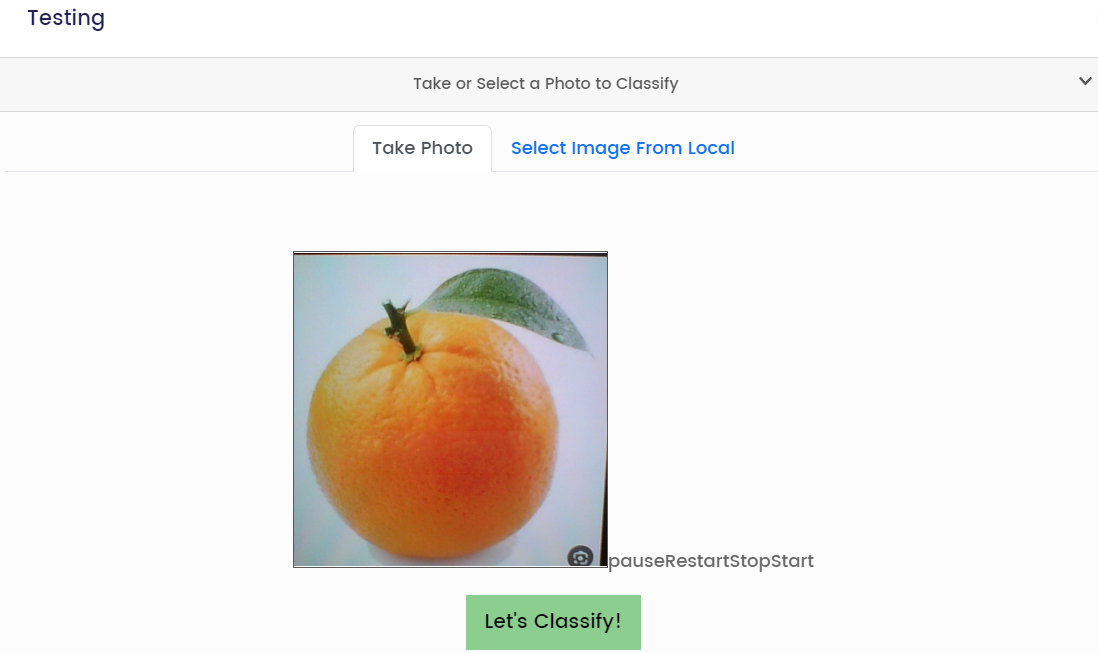
\includegraphics[width=\linewidth]{Chapters/Chapter_7/images/quality_check.png}
    \subcaption{Quality Check}
  \end{minipage}

  \vspace{0.5cm} % Adjust the vertical space between the images

  \begin{minipage}[b]{0.6\linewidth}
    \centering
    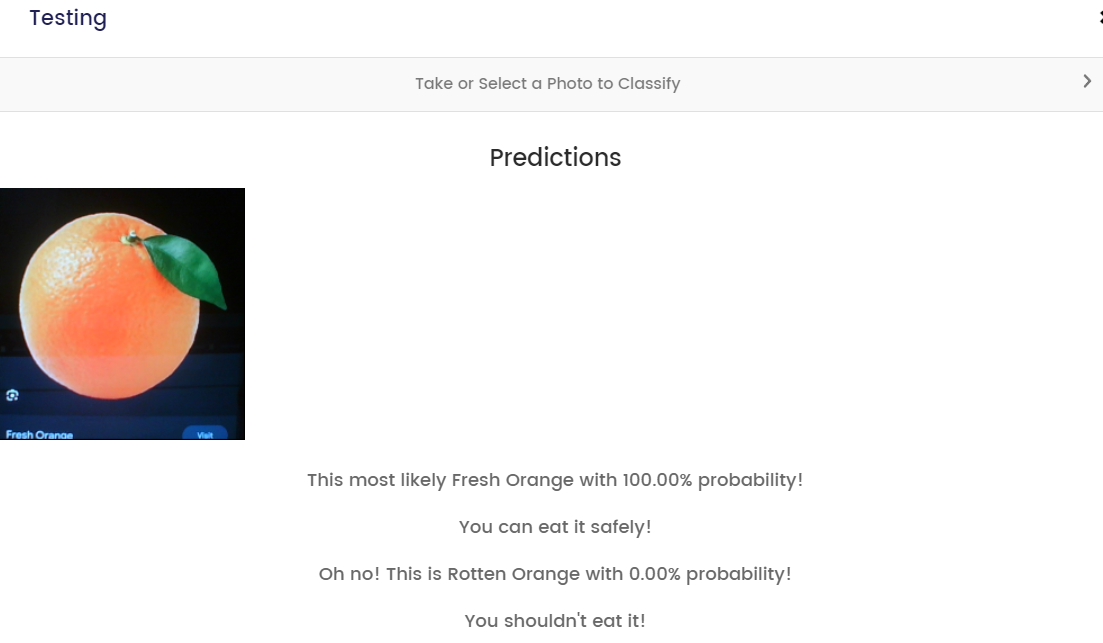
\includegraphics[width=\linewidth]{Chapters/Chapter_7/images/quality_check_result.png}
    \subcaption{Quality Check results}
  \end{minipage}
  
  \caption{Model Output}
  
  \label{fig:figure7_2}
\end{figure}
\noindent {Whenever an user wants to check whether the quality of the product is good or bad he can check that using an ML model,after checking the model is giving output as fresh if the fruit is in good condition and if not then the model is giving output as rotten.\par}
\noindent{The first diagram Figure \ref{fig:figure7_2}(A) is used to show how we can show the product to our camera sensor and after clicking on the let's clearift button it gives the result shown in the second diagram Figure i.e.\ref{fig:figure7_2}(B)}








\begin{figure}[htbp]
    \centering
    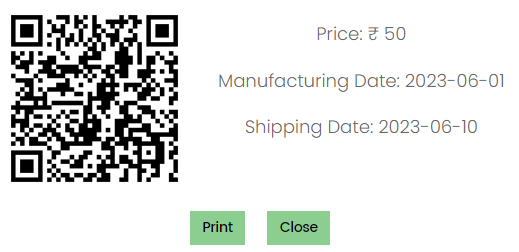
\includegraphics[width=0.7\textwidth]{Chapters/Chapter_7/images/Screenshot.png}
    \caption{Product Label }
    \label{fig:figure7_3}
    \end{figure}
\noindent {The product label shown in Figure \ref{fig:figure7_3} will provide the details of the product like the price,manufacturing date,shipping date etc.Also user can get a printed invoice of the price details\par}
\begin{figure}[htbp]
    % \centering
    \raggedright %
    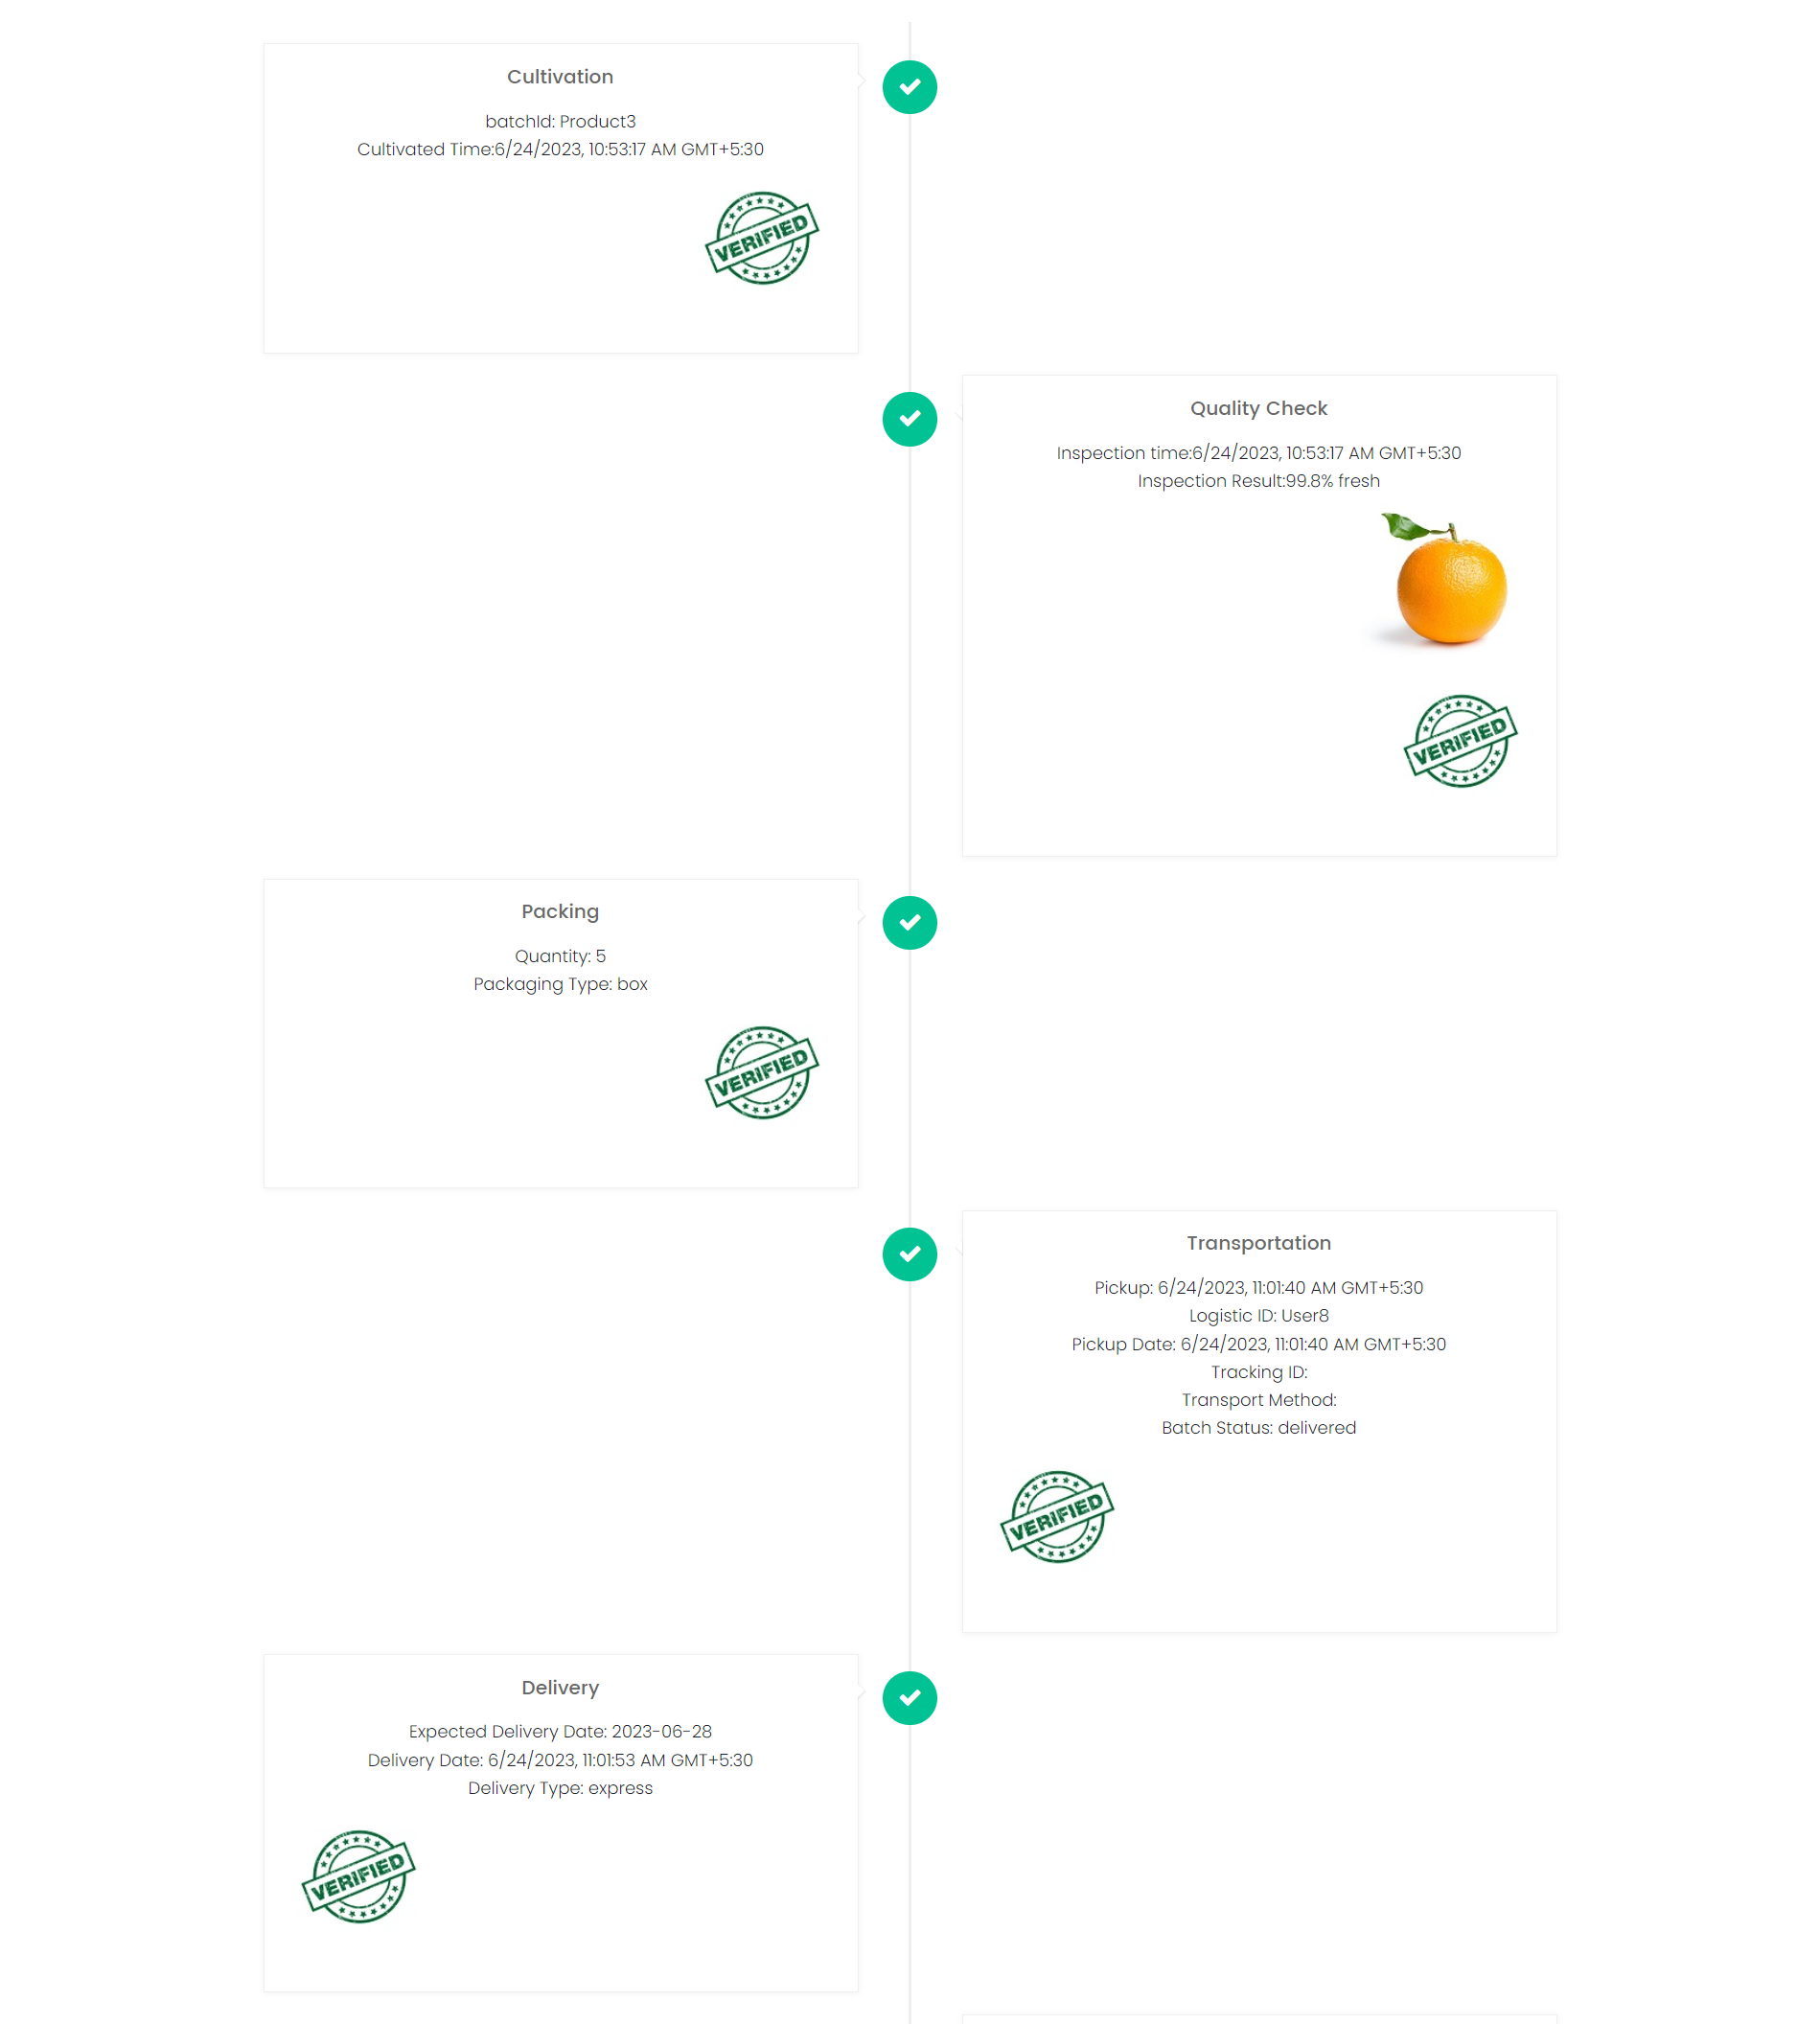
\includegraphics[width=1.2\textwidth]{Chapters/Chapter_7/images/veified.png}
    \caption{Product Timeline}
    \label{fig:figure7_4}
    \end{figure}
\noindent{The product timeline displayed in  Figure \ref{fig:figure7_4}  represents the progress and various stages of a product lifecycle in a supply chain system. The timeline showcases the different activities and events that occur during the cultivation, packaging, transportation, delivery, and marketing of a batch.

Here is a breakdown of the different sections in the batch timeline:

Cultivation: This section displays information related to the cultivation process. It includes details such as the batch ID, cultivation time, and a verification status.

Quality Check: This section represents the quality inspection stage. It shows the inspection time, inspection result, and verification status.

Packing: In this section, information about the packaging process is presented. It includes details like quantity, packaging type, and a verification status.

Transportation: This section focuses on the transportation of the batch. It provides information about the logistics involved, including the logistic ID, pickup date, tracking ID, transport method, and verification status.

Delivery: This section showcases the delivery stage of the batch. It includes details such as the expected delivery date, actual delivery date, delivery type, and verification status.

Marketing: This section represents the marketing activities related to the batch. 

Distribution: The last section,  display information about the distribution of the batch to consumers or retailers.

Each section in the timeline is presented with a timeline badge that indicates the status of that particular stage. A green badge with a checkmark represents a successful completion, while a red badge with an "X" indicates a failure or incomplete stage.

Overall, the batch timeline provides a visual representation of the product journey through the different stages of the supply chain, allowing users to track and monitor its progress.}
% \noindent{ The first diagram is used to show how we can show the fruit to our camera sensor and after clicking on the let's clearift button it gives the result shown in the second diagram i.e.Quality Check Results}
\vspace*{0.5cm}
\vspace*{0.5cm}
\section{Conclusion}
\noindent{In conclusion, a noteworthy development in the agriculture sector is the adoption of a blockchain-based farming system that combines supply chain management with machine learning algorithms to track and evaluate food quality. By ensuring transparency, traceability, and improved food safety, this novel concept transforms conventional farming methods.

The solution gives customers access to an immutable, decentralised ledger of all farming and supply chain activity by utilising blockchain technology. The ability to trace the path of their food from farm to table gives consumers the power to make knowledgeable decisions about the products they buy. The blockchain's immutability shields users from fraud, manipulation, and the introduction of fake items into the supply chain.
The system is further advanced because to the incorporation of machine learning models. These algorithms are able to analyse a variety of factors, including farming methods, environmental factors, and quality indicators, to evaluate the overall quality of the food by utilising enormous amounts of data. This enables prompt responses to reduce these risks and aids in the identification of potential hazards like contamination or spoiling. In the end, it makes sure that consumers have access to high-quality, safe food products.
All parties involved will profit greatly from the farming system's integration of blockchain and machine learning. Farmers may boost productivity, allocate resources more efficiently, and obtain insights into their farming practises. Distributors and retailers may increase customer trust while reducing waste and managing their inventory more effectively. On the other side, customers can relax knowing that they have open access to information on the food they eat.

Overall, the  blockchain-based farming system augmented by machine learning system raises industry standards for food safety, supply chain effectiveness, and consumer empowerment. It is a key step towards creating a food ecosystem that is safer and more sustainable, and it encourages everyone to take responsibility for their actions.









}
% ----------------------------
% Methodology
% ----------------------------

\section{Future Scope}
\noindent {The integration of blockchain-based farming systems with supply chain management and machine learning algorithms opens up a promising future for the agriculture industry. Here are some potential futurescopes for this innovative concept:

1. Enhanced Food Safety and Quality Assurance: As the technology continues to evolve, the integration of blockchain and machine learning can further enhance food safety and quality assurance measures. Advanced sensors and IoT devices can be integrated into the system to continuously monitor and collect real-time data on various parameters such as temperature, humidity, and soil conditions. This data can be analyzed by machine learning models to detect potential risks and ensure proactive interventions, thereby minimizing the occurrence of foodborne illnesses and maximizing food quality.

2. Expansion of Traceability and Certification: The blockchain-based farming system can extend its traceability capabilities by incorporating smart contracts and digital certifications. Smart contracts can automatically verify and enforce compliance with specific farming standards and regulations. Digital certifications, issued through blockchain, can provide a trustworthy and immutable record of organic, fair trade, or other specific product attributes. This expansion of traceability and certification will empower consumers with even more information about the origin, production practices, and authenticity of the food they purchase.

3. Integration with IoT and Automation: The integration of the farming system with the Internet of Things (IoT) and automation technologies holds immense potential. IoT devices such as drones, sensors, and autonomous machinery can be used to collect data, monitor crop health, and automate farming processes. These devices can interface with the blockchain system, recording and verifying data in real-time, while machine learning algorithms can analyze the data to optimize resource allocation, predict crop yields, and enable more efficient farming practices.

4. Consumer Engagement and Education: The blockchain-based farming system can serve as a platform for consumer engagement and education. Through mobile applications or web interfaces, consumers can access detailed information about the food they consume, including farming practices, environmental impact, and nutritional profiles. Educational resources, such as tutorials on sustainable farming or healthy eating, can be integrated into the system, promoting awareness and empowering consumers to make conscious food choices.

5. Global Collaboration and Standards: The adoption of blockchain-based farming systems can foster global collaboration and the establishment of common standards in the agriculture industry. By providing a transparent and decentralized platform, stakeholders from different regions and countries can collaborate, share best practices, and collectively work towards sustainable and efficient food production. This collaboration can lead to the development of globally recognized standards for farming practices, supply chain management, and quality assurance, promoting harmonization and trust across international markets.

In conclusion, the future of blockchain-based farming systems combined with supply chain management and machine learning is promising. With continued advancements and innovations, we can expect improved food safety, expanded traceability, increased automation, enhanced consumer engagement, and global collaboration in the agriculture industry. This technology-driven future holds the potential to create a more sustainable, transparent, and secure food ecosystem for the benefit of all stakeholders involved.}

